\documentclass[11pt,a4paper]{article}

\usepackage[utf8]{inputenc}
\usepackage[T1]{fontenc}
\usepackage[french]{babel}
\usepackage[a4paper,margin=2.4cm]{geometry}
\usepackage{graphicx}
\usepackage{booktabs}
\usepackage{array}
\usepackage{xcolor}
\usepackage{caption}
\usepackage{enumitem}
\usepackage{fancyhdr}
\usepackage{titlesec}
\usepackage[hidelinks]{hyperref}

\graphicspath{{figures/}}
\definecolor{nblue}{HTML}{1D3A6B}
\definecolor{acc}{HTML}{2563EB}

\titleformat{\section}{\Large\bfseries\color{nblue}}{\thesection}{0.6em}{}
\titleformat{\subsection}{\large\bfseries\color{acc}}{\thesubsection}{0.6em}{}
\setlength{\parskip}{0.5em}

\pagestyle{fancy}\fancyhf{}
\lhead{\small\color{nblue}Analyse NLP des rapports d'incidents ASRS}
\rhead{\small\thepage}
\renewcommand{\headrulewidth}{0.4pt}
\captionsetup{font=small,labelfont={bf,color=nblue}}

\newenvironment{narr}{%
  \begin{list}{}{\setlength{\leftmargin}{1.2em}\setlength{\rightmargin}{1.2em}}\item[]%
  \small\itshape\color{nblue}\guillemotleft~}{~\guillemotright\end{list}}

\begin{document}

% ---------- TITLE ----------
\begin{titlepage}
\centering
\vspace*{1.3cm}
{\small\color{acc}\textbf{AÉRONAUTIQUE \;|\; PROJET A3 \;|\; NLP · CLASSIFICATION · CLUSTERING}}\\[1.0cm]
{\color{nblue}\Huge\bfseries Analyse NLP des rapports\\[0.3cm] d'incidents de sécurité aérienne\par}
\vspace{0.45cm}
{\large Extraction des causes récurrentes, classification des anomalies\\ et détection de signaux faibles sur la base \textbf{NASA ASRS}\par}
\vspace{0.30cm}
{\itshape Rapport technique d'ingénierie\par}
\vspace{0.5cm}
{\large\bfseries TIDJANI Mehdi \quad\textbullet\quad FEUDJEU II LA GRACE \quad\textbullet\quad OUEDRAOGO Martin\par}
\vspace{0.8cm}
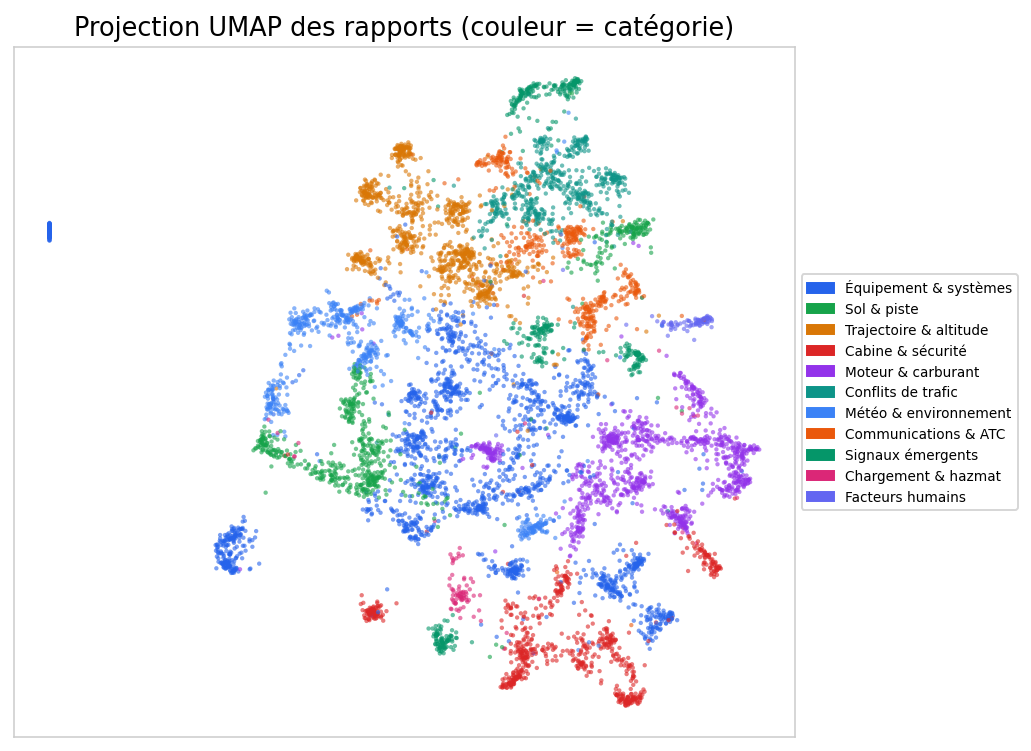
\includegraphics[width=0.90\textwidth]{scatter.png}\\[0.2cm]
{\small\itshape Projection sémantique des 125\,763 rapports, colorée par catégorie d'incident}
\vfill
\begin{tabular}{rl}
\textbf{Jeu de données} & NASA ASRS — 125\,763 rapports (2002–2025)\\
\textbf{Cadre} & Projet A3 — équipe de 3 étudiants \;|\; 3–4 semaines\\
\textbf{Livrables} & Pipeline NLP · Dashboards (Streamlit \& React) · Rapport\\
\textbf{Dépôt} & \url{https://github.com/devMehdi485/asrs-ml}\\
\end{tabular}
\vspace{0.8cm}
\end{titlepage}

% ---------- ABSTRACT ----------
\thispagestyle{empty}
\vspace*{2cm}
\begin{abstract}
\noindent Ce rapport présente la conception et l'évaluation d'une chaîne de traitement
automatique du langage naturel (NLP) destinée à exploiter 125\,763 rapports d'incidents en
texte libre de la base \emph{Aviation Safety Reporting System} (ASRS). La démarche est
guidée par les caractéristiques mesurées du corpus — texte rédigé librement, vocabulaire
abrégé et hétérogène, déséquilibre marqué des catégories d'anomalies, apparition de risques
nouveaux au fil du temps — et chaque décision méthodologique est présentée comme une réponse
à une difficulté identifiée dans les données, puis évaluée par ses conséquences sur les
résultats. La chaîne combine un prétraitement linguistique, une vectorisation (TF-IDF,
word2vec, embeddings de phrases), une réduction de dimension (UMAP), un regroupement
(comparaison K-Means / HDBSCAN), une modélisation de sujets (LDA) et une classification
supervisée (régression logistique, SVM). Les principaux résultats quantitatifs sont :
81 thèmes (silhouette de 0,590 pour HDBSCAN contre 0,382 pour K-Means), un score F1 pondéré
de 0,615 en classification, une cohérence $c_v$ de 0,57 pour le modèle LDA, et l'isolement
d'un ensemble de rapports atypiques correspondant à des risques émergents.

\bigskip
\noindent\textbf{Mots-clés :} traitement du langage naturel, sécurité aérienne, ASRS,
regroupement de textes, modélisation de sujets, classification, détection d'anomalies.
\end{abstract}
\newpage

\tableofcontents
\newpage

% ---------- 1 ----------
\section{Contexte et problématique}

La base \emph{Aviation Safety Reporting System} (ASRS) regroupe des rapports d'incidents
soumis volontairement par les acteurs du transport aérien. L'essentiel de l'information y est
contenu dans un \textbf{champ de texte libre} décrivant l'événement. Le présent travail porte
sur un export de 125\,763 rapports (2002–2025) ; les champs textuels sont renseignés à
100\,\% et les métadonnées exploitées sont quasi complètes (type d'anomalie 99,7\,\%, phase
de vol 95,9\,\%, type d'aéronef 98,9\,\%, date 100\,\%).

La difficulté centrale est que cette information n'est pas structurée et qu'un volume de cet
ordre n'est pas traitable manuellement. Le problème d'ingénierie traité est donc le suivant :
\textbf{concevoir une chaîne de traitement capable d'extraire automatiquement les causes
récurrentes d'incidents, de classifier les types d'anomalies et de détecter les signaux
faibles} (rapports atypiques potentiellement précurseurs), à partir du seul contenu textuel.
Le \textbf{NLP (Natural Language Processing)}, ensemble de méthodes d'analyse automatique du
langage écrit, fournit le cadre de cette chaîne.

% ---------- 2 ----------
\section{Objectifs}

\begin{enumerate}[leftmargin=1.5em]
  \item Extraire automatiquement les thèmes d'incidents récurrents, sans nomenclature
  prédéfinie.
  \item Prédire la catégorie d'anomalie d'un rapport à partir de son texte.
  \item Détecter les rapports atypiques susceptibles de signaler des risques émergents.
\end{enumerate}

% ---------- 3 ----------
\section{Démarche méthodologique}

La méthodologie n'est pas un catalogue d'algorithmes : chaque composant a été retenu en
réponse à une difficulté observée dans le corpus ASRS. Cette section suit cette logique, en
partant des propriétés mesurées des données pour en déduire les choix de traitement et leurs
conséquences.

\subsection{Propriétés du corpus et prétraitement}
Trois propriétés du corpus déterminent l'ensemble des décisions ultérieures. D'abord, les
récits sont rédigés librement : un même événement opérationnel est décrit avec des
formulations très variables. Ensuite, l'anonymisation introduite par la NASA remplace noms et
lieux par des marqueurs (\texttt{ZZZ}, \texttt{XXX}) qui, présents dans la quasi-totalité des
rapports, constitueraient les jetons les plus fréquents du corpus s'ils étaient conservés.
Enfin, le vocabulaire technique est fortement abrégé et orthographié de manière inconsistante
(\texttt{rwy} pour \emph{runway}, \texttt{eng} pour \emph{engine}).

La deuxième propriété impose un prétraitement avant toute statistique lexicale : retrait des
marqueurs d'anonymisation et d'un ensemble de termes omniprésents et non discriminants
(« aircraft », « flight »), puis lemmatisation pour regrouper les variantes flexionnelles
(« engine », « engines »). Sans ce traitement, les regroupements refléteraient la présence de
marqueurs plutôt que la nature des incidents. La validité de ce nettoyage est confirmée a
posteriori par l'extraction de termes distinctifs par cluster (c-TF-IDF, \S\,3.3), qui
restitue un vocabulaire spécifique aux incidents (par exemple « hydraulic, pump ») et non le
vocabulaire générique du domaine.

\subsection{Représentation des récits}
La tâche de classification et la nomination des thèmes exigent une représentation dont on
puisse lire les termes responsables d'une décision. Le \textbf{TF-IDF} (\emph{Term Frequency –
Inverse Document Frequency}), qui pondère chaque mot par sa fréquence locale et l'inverse de
sa fréquence dans le corpus, répond à ce besoin : il atténue le socle lexical commun
(phraséologie, procédures) que partagent tous les rapports et fait ressortir les termes
décisifs et peu fréquents qui caractérisent un incident particulier. Cette représentation
sera réutilisée comme entrée des modèles de classification (\S\,3.4), dont elle conditionne
l'interprétabilité.

Le TF-IDF ne peut toutefois pas rapprocher deux écritures d'un même concept : \texttt{rwy} et
\texttt{runway} y forment deux dimensions indépendantes. L'ampleur de cette limite a été
quantifiée en entraînant un modèle \textbf{word2vec} (représentation vectorielle apprise par
co-occurrence) sur le corpus : les plus proches voisins obtenus
(\texttt{runway}~$\to$~\texttt{rwy} à 0,84 ; \texttt{weather}~$\to$~\texttt{thunderstorm} à
0,76 ; tableau~\ref{tab:w2v}) montrent que la synonymie de domaine est massive et qu'une
représentation purement lexicale la manque.

Cette observation conduit, pour le regroupement, à représenter chaque rapport par un
\textbf{embedding} (vecteur numérique encodant le sens global du texte) produit par un
\textbf{Sentence Transformer} (modèle de phrases pré-entraîné, \texttt{all-MiniLM-L6-v2}). La
raison est directement liée à la première propriété du corpus : deux rapports décrivant une
même situation — par exemple une approche non stabilisée écrite « we were high and fast on
final » ou « the approach became unstabilized and we went around » — ne partagent presque
aucun mot et seraient jugés distants par TF-IDF, alors que leurs embeddings sont proches. La
conséquence sur les résultats est mesurable : le regroupement opéré sur les embeddings atteint
une silhouette de 0,590 (\S\,3.3), nettement supérieure à ce que permettrait une
représentation par mots-clés. Le TF-IDF est conservé en parallèle, non pour le regroupement,
mais parce que son caractère interprétable reste nécessaire à la classification et à
l'étiquetage.

\subsection{Réduction de dimension et regroupement}
Les embeddings comportent 384 dimensions pour 125\,763 rapports. À cette dimensionnalité, les
distances euclidiennes se concentrent et perdent leur pouvoir discriminant, ce qui dégrade les
méthodes de regroupement par densité. Une réduction préalable est donc appliquée au moyen
d'\textbf{UMAP} (\emph{Uniform Manifold Approximation and Projection}), qui projette les
vecteurs dans un espace de faible dimension en préservant les voisinages locaux ; ce dernier
point écarte une réduction linéaire (ACP), qui ne conserverait pas la structure locale des
groupes sémantiques. Cette réduction rend le regroupement par densité applicable et fournit la
projection bidimensionnelle utilisée pour la visualisation.

Le nombre de types d'incidents n'est pas connu a priori, et l'examen du corpus révèle une
distribution très inégale : quelques thèmes massifs (l'équipement représente 43,8\,\% des
rapports, \S\,4) coexistent avec une longue traîne de thèmes rares, et une part substantielle
des récits sont atypiques ou hors-sujet. Ces propriétés orientent le choix de l'algorithme.
\textbf{K-Means} impose de fixer le nombre de groupes et attribue chaque rapport à un groupe,
y compris les récits atypiques, ce qui dilue les thèmes. \textbf{HDBSCAN} (\emph{Hierarchical
Density-Based Spatial Clustering of Applications with Noise}) déduit le nombre de groupes de
la densité, admet des groupes de tailles très différentes et étiquette comme « bruit » les
points isolés. La comparaison des deux approches sur les mêmes données (tableau~\ref{tab:clust})
départage : HDBSCAN obtient une silhouette de 0,590 et un indice de Davies-Bouldin de 0,575,
contre 0,382 et 0,945 pour K-Means. HDBSCAN est donc retenu. Deux conséquences en découlent.
D'une part, les 32\,\% de points classés « bruit » ne sont pas écartés mais réutilisés en
entrée de la détection d'anomalies (\S\,3.4), ce qui transforme une limite apparente du
regroupement en ressource. D'autre part, la concordance entre les 81 thèmes obtenus et les
catégories d'anomalies codées par les analystes est faible (pureté de 0,165) : ce résultat
n'indique pas une erreur mais une différence de granularité, les thèmes issus du texte étant
plus fins que la nomenclature officielle (un code « équipement » se subdivise en hydraulique,
train, circuit d'huile, électrique, etc.).

L'étiquetage des thèmes pose un problème spécifique : les mots les plus fréquents d'un groupe
sont le vocabulaire commun à tous les groupes et ne le caractérisent pas. Les termes
distinctifs sont donc extraits par \textbf{c-TF-IDF}, variante du TF-IDF appliquée en traitant
chaque groupe comme un document unique. Les 81 thèmes ainsi nommés ont ensuite été regroupés
manuellement en 11 catégories métier afin d'offrir un niveau de lecture agrégé.

\subsection{Modélisation des sujets, classification et détection d'anomalies}
Un regroupement attribue chaque rapport à un thème unique, alors que les récits ASRS
combinent fréquemment plusieurs problèmes (par exemple une déviation météorologique
entraînant un écart d'altitude puis une difficulté de communication). Pour représenter cette
multiplicité, une modélisation \textbf{LDA} (\emph{Latent Dirichlet Allocation}), qui décrit
chaque document comme un mélange de sujets, est ajoutée en complément ; la cohérence $c_v$ de
ses sujets atteint 0,57.

La classification vise à reconstituer la catégorie d'anomalie à partir du texte complet du
rapport, dans une perspective de pré-tri automatique des nouveaux rapports. Les entrées étant
des vecteurs TF-IDF creux et de grande dimension, des modèles linéaires sont adaptés à cette
configuration : la \textbf{régression logistique} (estimation de probabilités d'appartenance)
et le \textbf{SVM linéaire} (\emph{Support Vector Machine}, séparation à marge maximale). Leur
caractère auditable — la possibilité d'identifier les termes déterminant une prédiction — est
un critère retenu dans un contexte de sécurité. Le champ d'anomalie étant en pratique
multi-valué, il a été ramené à la catégorie principale (huit classes majoritaires) ; cette
simplification borne la performance atteignable et explique en partie la difficulté sur les
classes rares.

Enfin, les risques émergents ne disposent d'aucune étiquette et sont absents au début de la
période étudiée ; ils ne peuvent donc être recherchés ni par apprentissage supervisé ni par
mots-clés prédéfinis. La détection s'appuie en conséquence sur une méthode non supervisée,
l'\textbf{Isolation Forest}, qui isole les points les plus éloignés de la masse dans l'espace
des représentations, complétée par les points « bruit » d'HDBSCAN. Cette approche fait
remonter des récits atypiques indépendamment de leur vocabulaire.

% ---------- 4 ----------
\section{Résultats}

\subsection{Structure thématique}
Le regroupement produit 81 thèmes, agrégés en 11 catégories (figure~\ref{fig:cat}). La
catégorie \emph{Équipement \& systèmes} concentre 43,8\,\% des rapports, devant
\emph{Sol \& piste} (13,3\,\%) et \emph{Trajectoire \& altitude} (7,8\,\%). La prédominance de
la première catégorie s'interprète comme une propension élevée des équipages à signaler les
dysfonctionnements techniques plutôt que comme une fréquence de pannes ; elle indique un
gisement de données pertinent pour une politique de maintenance fondée sur l'analyse des
signalements.

\begin{figure}[h]\centering
  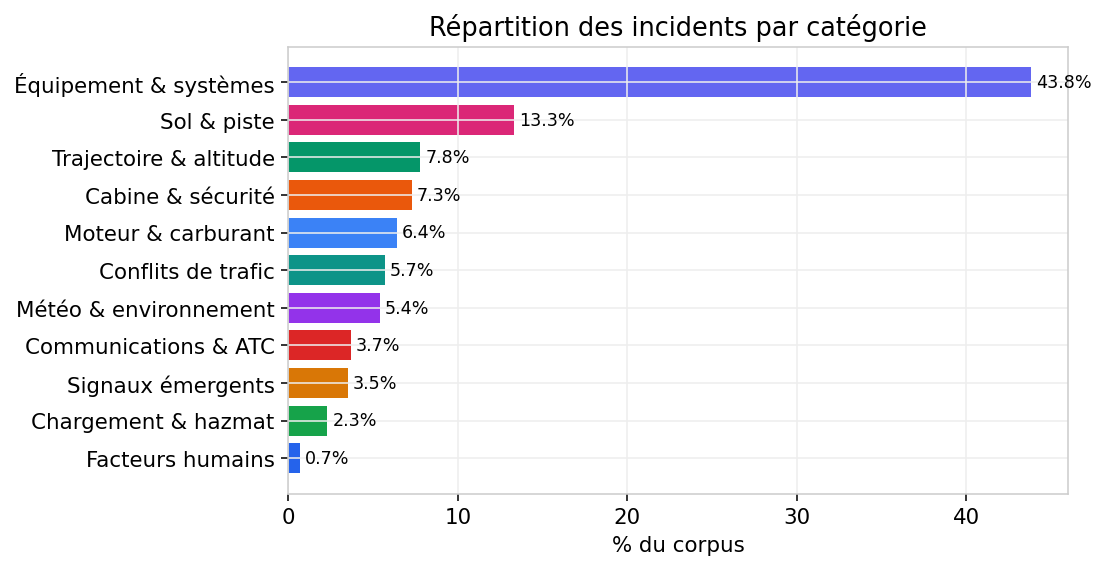
\includegraphics[width=0.80\textwidth]{categories.png}
  \caption{Répartition des rapports par catégorie (regroupement des 81 thèmes en 11 familles).}\label{fig:cat}
\end{figure}

\begin{figure}[h]\centering
  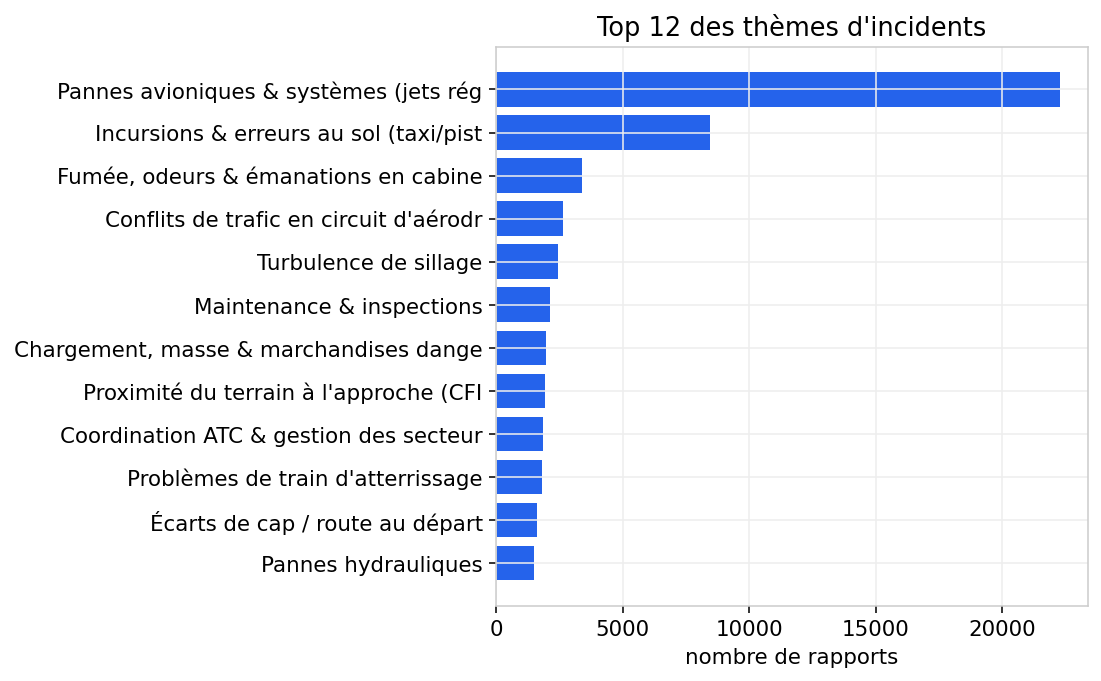
\includegraphics[width=0.80\textwidth]{top_themes.png}
  \caption{Douze thèmes les plus volumineux.}\label{fig:top}
\end{figure}

Les termes distinctifs extraits par c-TF-IDF (figure~\ref{fig:wc}) confèrent à chaque thème un
contenu identifiable, condition nécessaire à l'exploitation opérationnelle des résultats.

\begin{figure}[h]\centering
  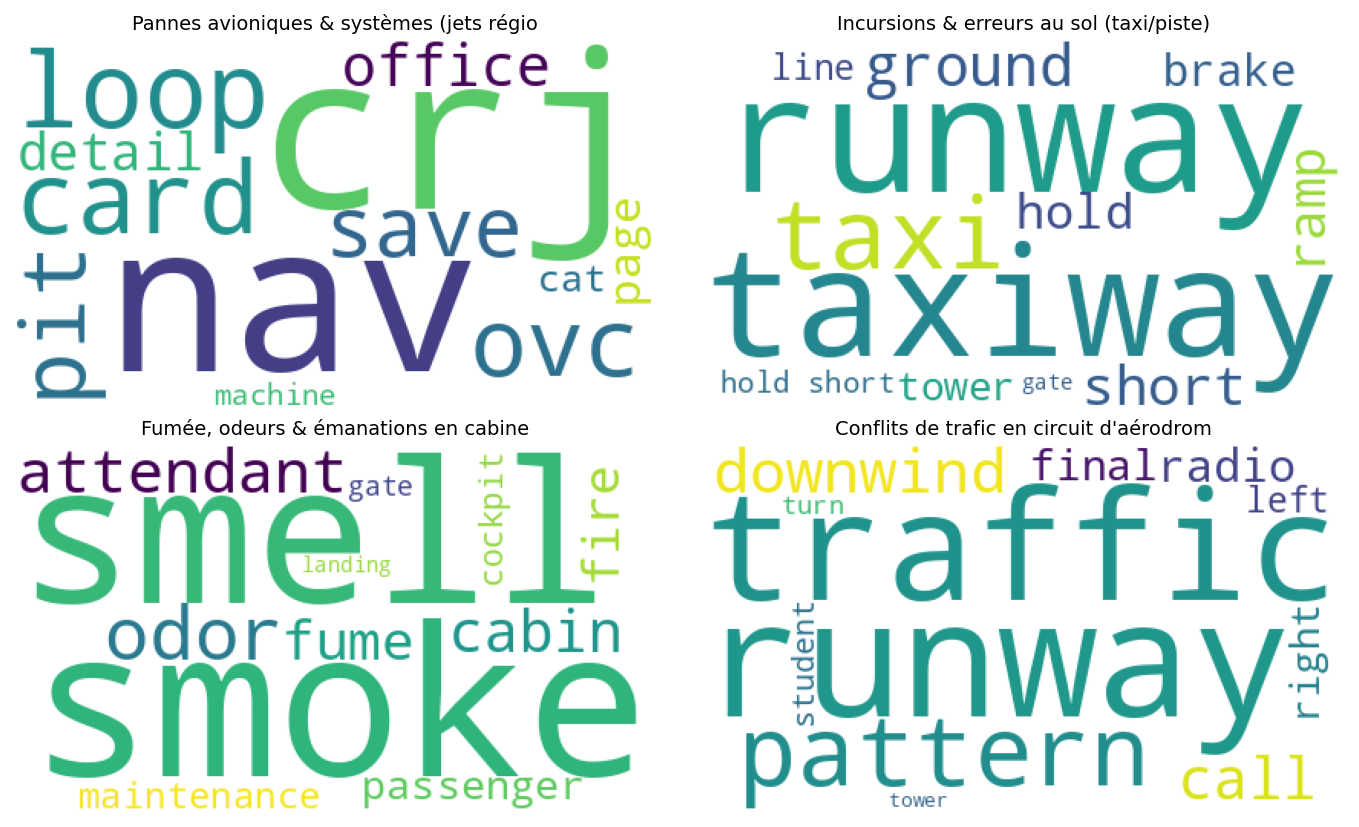
\includegraphics[width=0.92\textwidth]{wordclouds.png}
  \caption{Termes distinctifs (c-TF-IDF) des quatre principaux thèmes.}\label{fig:wc}
\end{figure}

\subsection{Évaluation du regroupement}
L'évaluation s'appuie sur trois indices internes : le \textbf{score de silhouette}
($-1$ à $1$ ; une valeur élevée traduit des groupes compacts et séparés), l'\textbf{indice de
Davies-Bouldin} (une valeur faible traduit une bonne séparation) et le \textbf{score de
Calinski-Harabasz}. Les valeurs obtenues (tableau~\ref{tab:clust}) établissent la supériorité
d'HDBSCAN sur ce corpus.

\begin{table}[h]\centering\small
\caption{Indices internes de qualité du regroupement.}\label{tab:clust}
\begin{tabular}{lrrrrr}
\toprule
\textbf{Algorithme} & \textbf{Groupes} & \textbf{Silhouette} & \textbf{Davies-Bouldin} & \textbf{Bruit} & \textbf{Pureté} \\
\midrule
K-Means & 15 & 0,382 & 0,945 & 0\,\% & 0,133 \\
HDBSCAN & 81 & 0,590 & 0,575 & 32\,\% & 0,165 \\
\bottomrule
\end{tabular}
\end{table}

La cohérence sémantique de la représentation est par ailleurs attestée par le modèle word2vec
(tableau~\ref{tab:w2v}), dont les voisinages reproduisent des relations de domaine
(abréviations, termes associés).

\begin{table}[h]\centering\small
\caption{word2vec — plus proches voisins (similarité cosinus) sur le corpus.}\label{tab:w2v}
\begin{tabular}{ll}
\toprule
\textbf{Terme} & \textbf{Plus proches voisins} \\
\midrule
\texttt{runway}   & rwy (0,84), taxiway (0,65), intersecting (0,59), midfield (0,59) \\
\texttt{engine}   & eng (0,69), feathered (0,57), magneto (0,54), crossbleed (0,54) \\
\texttt{weather}  & thunderstorm (0,76), storm (0,74), bkn (0,68), forecast (0,66) \\
\texttt{altitude} & alt (0,70), descended (0,67), descend (0,65), level (0,64) \\
\bottomrule
\end{tabular}
\end{table}

\subsection{Classification des anomalies}
Les performances sont mesurées par le score \textbf{F1} (moyenne harmonique de la précision et
du rappel), rapporté en moyenne non pondérée (\emph{macro}) et pondérée par les effectifs.

\begin{table}[h]\centering\small
\caption{Classification de la catégorie d'anomalie (8 classes, entrées TF-IDF).}\label{tab:clf}
\begin{tabular}{lrr}
\toprule
\textbf{Modèle} & \textbf{F1 macro} & \textbf{F1 pondéré} \\
\midrule
Régression logistique & 0,518 & 0,606 \\
SVM linéaire & 0,517 & 0,615 \\
\bottomrule
\end{tabular}
\end{table}

Le SVM linéaire atteint un F1 pondéré de 0,615. L'écart entre F1 macro (0,517) et F1 pondéré
confirme l'effet du déséquilibre des classes : les catégories au vocabulaire spécifique sont
bien reconnues (\emph{ATC Issue}, F1\,=\,0,76 ; \emph{NMAC}, 0,69 ; \emph{Aircraft Equipment
Problem Critical}, 0,67), tandis que les classes minoritaires et les rapports multi-anomalies
abaissent la moyenne macro.

% ---------- 5 ----------
\section{Analyse des tendances et des signaux faibles}

L'horodatage des rapports permet de mesurer l'évolution de chaque thème
(figures~\ref{fig:vol} et~\ref{fig:heat}). Plusieurs thèmes présentent une progression
significative sur la période récente. Les \textbf{incursions et erreurs au sol} augmentent, ce
qui est cohérent avec la densification du trafic au sol et l'augmentation mécanique des
situations de croisement sur les aires de manœuvre. Les \textbf{événements de fumée ou
d'odeur en cabine} progressent également, de même que les rapports relatifs aux
\textbf{marchandises dangereuses}, ce dernier point étant cohérent avec la croissance du fret.

\begin{figure}[h]\centering
  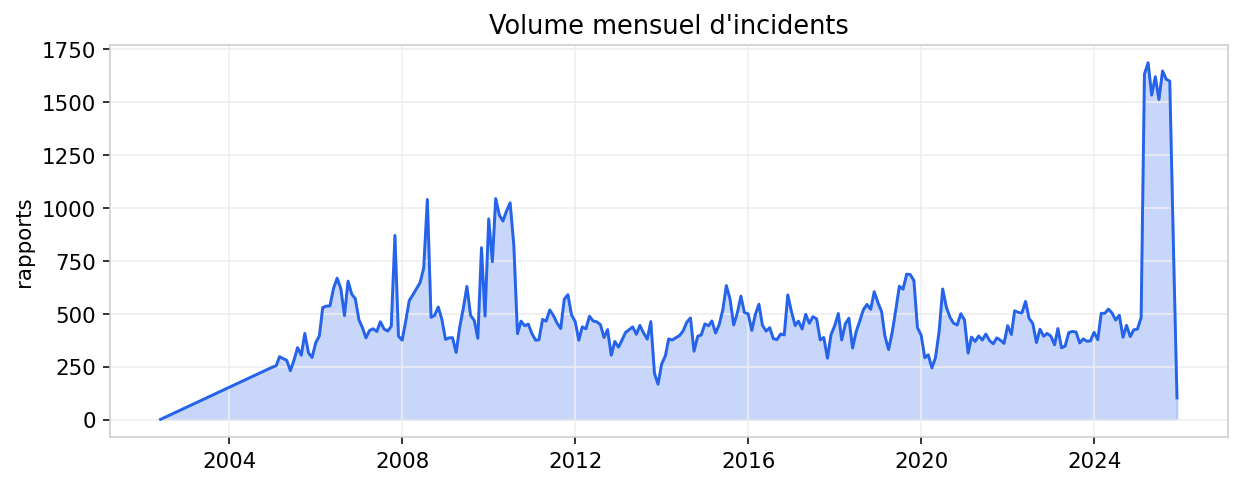
\includegraphics[width=0.84\textwidth]{temporal_volume.png}
  \caption{Volume mensuel de rapports (2002–2025).}\label{fig:vol}
\end{figure}
\begin{figure}[h]\centering
  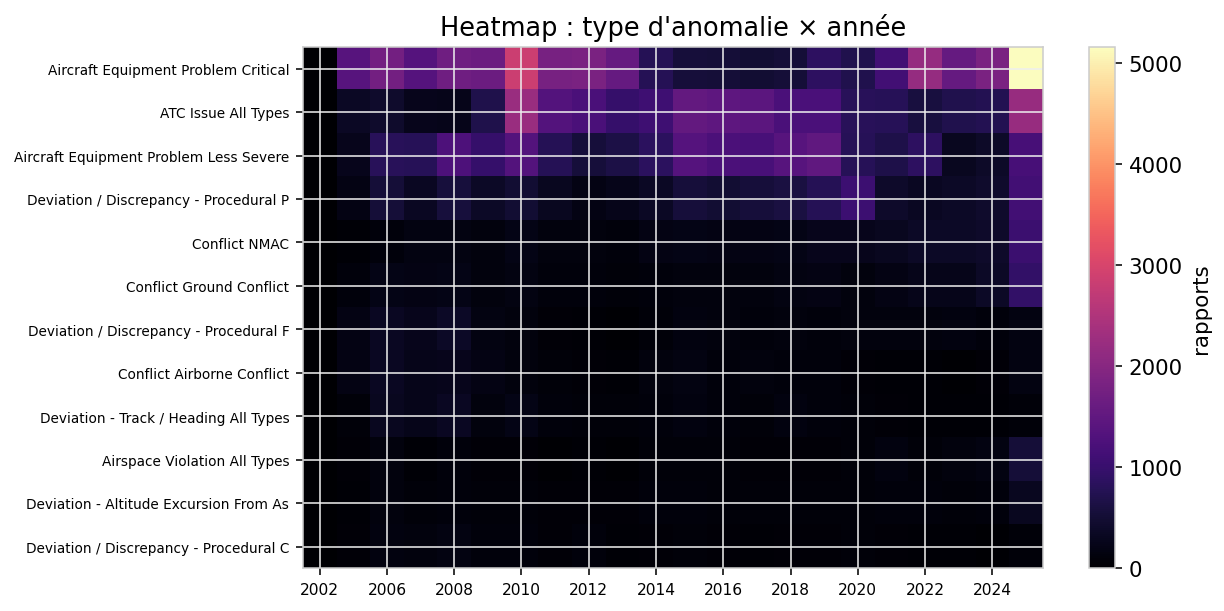
\includegraphics[width=0.84\textwidth]{heatmap.png}
  \caption{Répartition des principales anomalies par année.}\label{fig:heat}
\end{figure}

La détection d'anomalies isole un ensemble de rapports atypiques dont l'examen fait apparaître
des thématiques rares et récentes : rencontres avec des drones, brouillage du signal GPS,
batteries au lithium. Ces thématiques étaient quasi absentes en début de période, ce qui
illustre la capacité de l'approche à faire émerger des risques non anticipés. Le rapport
suivant, classé parmi les plus atypiques, en est représentatif :

\begin{narr}
Approach control advised there was unauthorized drone use in the area\ldots I observed a
drone pass just left of the aircraft, approximately 20 feet from our left wing.
\end{narr}

\noindent L'intérêt opérationnel de cette détection tient au fait que de tels rapports,
minoritaires, ne seraient pas identifiés par une revue manuelle ni par une recherche par
mots-clés portant sur des risques connus.

% ---------- 6 ----------
\section{Limites et perspectives}

L'interprétation des résultats est soumise à plusieurs réserves, toutes liées aux propriétés
des données. Le déséquilibre des classes pénalise la reconnaissance des anomalies rares, comme
l'indique l'écart entre F1 macro et F1 pondéré. L'anonymisation supprime un contexte
potentiellement informatif (lieux, opérateurs). Le caractère volontaire de l'ASRS implique
que le corpus reflète les incidents \emph{signalés} et non l'ensemble des incidents, ce qui
limite la portée statistique des fréquences observées. Enfin, le thème relatif à l'équipement
reste hétérogène, conséquence du caractère généraliste du modèle d'embeddings utilisé.

Plusieurs prolongements répondraient directement à ces limites. L'emploi d'embeddings
ré-entraînés sur un corpus aéronautique améliorerait la séparation des thèmes techniques. Une
approche de modélisation de sujets fondée sur les embeddings (de type BERTopic) unifierait
regroupement et nomination. Une formulation multi-étiquettes de la classification rendrait
compte des rapports relevant de plusieurs anomalies. Le croisement des rapports atypiques avec
des données externes (trafic, conditions météorologiques) permettrait enfin d'évaluer leur
valeur prédictive.

% ---------- 7 ----------
\section{Conclusion}

Le travail décrit une chaîne de traitement complète permettant d'exploiter
automatiquement 125\,763 rapports d'incidents en texte libre. Les choix méthodologiques ont
été déterminés par les propriétés mesurées du corpus et évalués par leurs effets sur les
résultats : 81 thèmes interprétables (silhouette de 0,590), une classification atteignant un
F1 pondéré de 0,615, une modélisation de sujets de cohérence $c_v = 0{,}57$, et l'isolement
d'un ensemble de rapports atypiques correspondant à des risques émergents. L'ensemble structure
une information jusque-là dispersée dans le texte et la rend exploitable pour l'analyse de la
sécurité aérienne, ouvrant la voie aux prolongements identifiés ci-dessus.

\vfill
\noindent\footnotesize\textit{Sources des données : NASA Aviation Safety Reporting System
(\url{https://asrs.arc.nasa.gov/}) et jeu équivalent sur Kaggle. Code, dashboards et
reproductibilité : \url{https://github.com/devMehdi485/asrs-ml}.}

\end{document}
